{\color{blue}
\section{Ablation Study}

To ensure that the architectural differences between DISCO and OE apart from the SPM and the heterogeneity do not make an impact in the kernels, we conduct an ablation study extending OE with DISCO's attributes and comparing the performance.

On the memory plane, DISCO has the SPM, the VWRs and an Scalar Register File shared among the PEs in a column.  The SRf will be exactly replicated in OE as it can be to see it's contribution to the performance on the architecture. For the SPM and VWRs, we can use the direct memory addressing of OE to only employ direct memory acceses so thath we completely remove the addrees computation overhead to see if this has a big implication on memoery to match the addr simplicity given by the SPM and the VWRs.

On the artihmetic plane, DISCo has heterogeneous PEs taking charge of specific operations such as memory accesses and loop control. We simulate a similar behaviour in OE, having PEs dedicated to only this specific tasks.

\subsection{Impact of the Scalar Register File}
\label{subsec:srf-ablation}

The experimental OE extension, matching DISCO capabilities, provides eight shared scalar registers per
column, accessible to the RCs in that column and initialized before kernel
execution. There are two versions of the kernel with different data stored in the SRF. The \emph{SRF Offsets} version stores address increments and reused parameters
in these registers while the \emph{SRF Base} version stores reusable base addresses to restore
matrix positions directly during traversal.


\begin{figure}
    \centering
    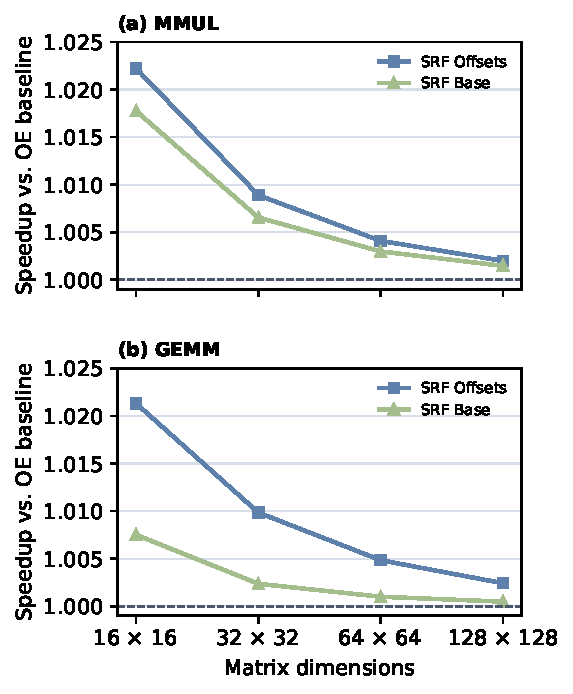
\includegraphics[width=\linewidth]{Figures/srf_ablation.pdf}
    \caption{Speedup over the original OE mapping for (a) MMUL and (b) GEMM.
    The horizontal dashed line denotes the OE baseline (1$\times$).}
    \label{fig:srf-ablation}
\end{figure}

Figure~\ref{fig:srf-ablation} summarizes the measured speedups, where total simulated cycles include static instruction-configuration costs and executed kernel cycles. Integrating the SRF reduces total cycles across all tested sizes for both MMUL and GEMM ($C = \alpha AB + \beta C$). In both kernels, sharing scalars, strides, and fused configuration schedules lowers control and address-management overhead, yielding speedups up to $1.022\times$ for MMUL and $1.021\times$ for GEMM on smaller matrices ($16\times16$). However, the overall performance impact remains minimum in all cases and decreases as the matrix size grows. While absolute cycle savings increase with problem size—driven by address-management reductions that scale with the number of output tiles—this benefit is quickly diluted by the raw compute scaling. Consequently, the impact of including an SRF becomes negligible for both workloads.

\subsection{Simplified Memory Addressing}
\label{subsec:simple-address}

Indirect memory operations in OE require the mapped program to form and update matrix addresses during execution. We estimate the cycle cost of simplifying this mechanism by replacing matrix loads and stores with column-shared direct-access pointers that advance by one word, requiring to arrange operands into sequential streams prior to kernel execution.

As shown in Figure~\ref{fig:simple-address-speedup}, replacing indirect addressing with direct-access streams removes two address-generation PCs from MMUL and four from GEMM, yielding peak speedups of $1.018\times$ and $1.023\times$ on smaller matrices ($16\times16$), respectively. GEMM achieves slightly higher gains across all sizes because its schedule contains additional removable address PCs. However, the performance impact remains modest overall and decreases with matrix size—falling to around $1.002\times$--$1.003\times$ at $128\times128$—as unchanged matrix arithmetic dominates execution.

Furthermore, this minor cycle reduction trades runtime address overhead for substantial memory bloat and preparation cost. Counting each element as a 32-bit word, the streamed layout expands memory footprint by $2.94\times$--$21.66\times$ for MMUL and $3.25\times$--$21.99\times$ for GEMM across sizes 16 to 128.

\subsection{Combined Impact of Simplified Addressing and Loop Control}
\label{subsec:combined-address-lcu}

We combine column-shared direct load/store pointers with specialized loop
control while retaining the original 16 compute PEs, 4$\times$4 toroidal
network, and 4$\times$4 output tiling. Five mappings are compared: the OE
baseline, Simple Address alone, one global LCU alone, and Simple Address
with either one global LCU or four synchronized row LCUs representing a
4$\times$5 organization. All MMUL and GEM
outputs match an independent reference at $N=16,32,64,128$; the direct
access sequences and final pointer positions also match the prepared streams.

Figure~\ref{fig:combined-address-lcu-speedup} shows that the combined
mapping reduces total modeled cycles from 4,644 to 4,299 (MMUL) and from
5,363 to 4,958 (GEM) at $N=16$, corresponding to 1.080$\times$ and
1.082$\times$ speedups. At $N=128$, it saves 135,277 and 138,361 cycles,
respectively, with speedups of 1.068$\times$ for both kernels. The gain
exceeds the sum of the separate gains: simplifying addresses makes two
MMUL and three GEM branch PCs control-only, allowing their LCU operations
to issue at the preceding PC boundary and eliminating repeated PE issue
cycles. These control savings recur across reduction iterations, so they
remain appreciable as $N$ grows. LCU offload alone cannot remove these PCs
because they also perform
address updates. One global LCU and four row LCUs produce identical cycle
counts and branch outcomes, so the four-LCU organization offers no modeled
throughput advantage for these synchronized loops. These figures include
PE and LCU instruction configuration but exclude host-side stream preparation;
the PE-to-LCU control and Rout sidebands remain simulator abstractions.

\begin{figure}[t]
    \centering
    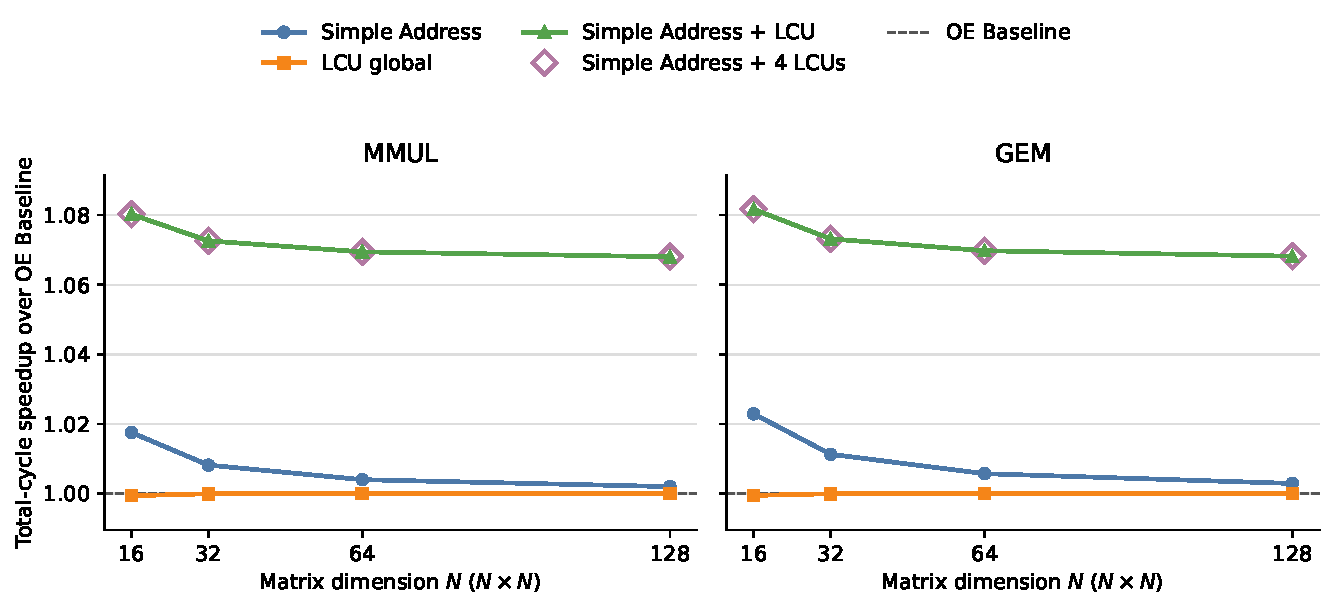
\includegraphics[width=\linewidth]{../benchmarks/DISCOvsOE/combined_architecture/combined_speedup.pdf}
    \caption{Total modeled-cycle speedup over the 4$\times$4 OE baseline for
    MMUL and GEM. The dashed line indicates equal performance. The one-LCU
    and four-LCU combined curves coincide at every matrix size.}
    \label{fig:combined-address-lcu-speedup}
\end{figure}
}
